In diesem Abschnitt wird auf den in \cite{hal02158423} vorgestellten, temporalen Algorithmus eingegangen.
Dieser besteht grundsätzlich aus den beiden Schritten: \nameref{ch:Content2:sec:Sorting} und  
\nameref{ch:Content2:sec:Retargeting}. Wir werden die gewonnenen Erkenntnisse (siehe Kapitel \ref{ch:Grundlagen})
nutzen um eine zeitlich stabile \nameref{ch:Content1:sec:blue noise} Fehlerverteilung im Bildraum zu erreichen.
Der benutzte \nameref{ch:Content1:sec:Path Tracer} benutzt zufällig generierte Anfangswerte 
(siehe \cite{matsumoto1998mersenne}). Der darauffolgende Schritt sortiert diese Anfangswerte anhand 
einer \nameref{ch:Content1:sec:blue noise} Textur, auf die mit Hilfe einer quasi-zufälligen Sequenz 
\ref{ch:Content1:sec:Quasi-Zufallsfolgen} zugegriffen wird. Bevor diese sortierten Anfangswerte 
zum Rendern des nächsten Bildes benutzt werden durchlaufen Sie noch eine Permutation 
(siehe Abschnitt \ref{ch:Content2:sec:Retargeting}).
Desweiteren sollte man beachten, dass für diesen Algorithmus Annahmen getroffen wurden, auf deren Ursache im darauffolgenden 
Abschnitt \ref{ch:Content2:sec:a Posteriori} eingegangen wird:
Der Algorithmus arbeitet Blockweise auf den Pixeln und erwartet, dass benachbarte
Pixel innerhalb dieses Blockes den selben Wert haben. Da wir einen temporalen Algorithmus haben, soll diese Annahme 
auch über mehrere gerenderte Bilder hinweg gelten. Es sollte also beachtet werden, dass der Algorithmus z.B. nicht 
für Objektkanten oder ruckartige Bewegungen (der Kamera oder Objekte) ausgelegt ist.

\begin{figure}[H]
    \begin{subfigure}{\textwidth}
        \centering 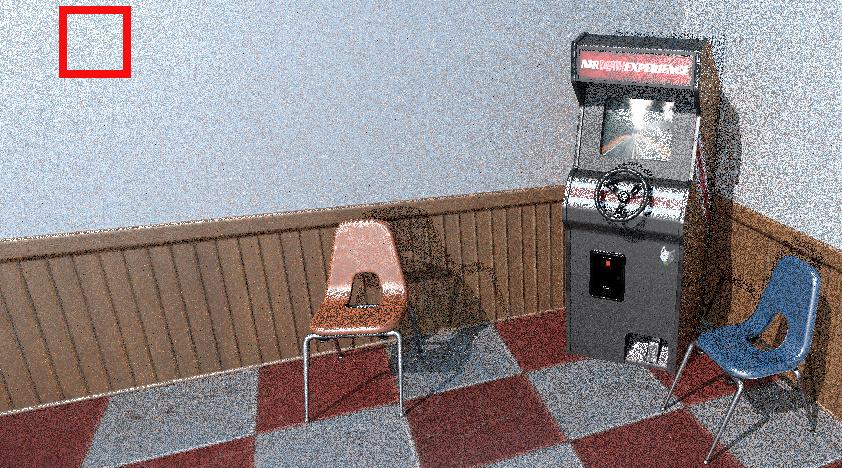
\includegraphics[width=0.7\linewidth]{content/TemporalerAlg/Bilder/WhiteNoise/white_noise_ausschnitt.png}
        \caption{Szene}
        \label{fig:Szene_Weißes Rauschen}
    \end{subfigure}
    \begin{subfigure}{0.5\textwidth}
        \centering 
\includegraphics[width=0.5\linewidth]{content/TemporalerAlg/Bilder/WhiteNoise/white_noise_64x64.jpg} 
        \caption{Szenenausschnitt}
        \label{fig:ausschnitt_Weißes_Rauschen}
    \end{subfigure}
    \begin{subfigure}{0.5\textwidth}
        \centering 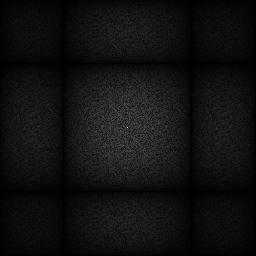
\includegraphics[width=0.5\linewidth]{content/TemporalerAlg/Bilder/WhiteNoise/white_noise_64x64_fourier.png}
        \caption{Fouriertransformierte des Ausschnitts}
        \label{fig:Fouriertransformierte_Weißes_Rauschen}
    \end{subfigure}
        \caption{Ausgangssituation; Erzeugtes Bild mit zufälligen Seeds ohne temp. Alg.}
        \label{fig:Path Tracer mit zufälligen Seeds}
\end{figure}

In Abbildung \ref{fig:Path Tracer mit zufälligen Seeds} sehen wir die Ausgabe des \nameref{ch:Content1:sec:Path Tracer}
mit zufälligen Anfangswerten(Mersenne-Twister) weder mit dem Sortier \ref{ch:Content2:sec:Sorting} noch dem 
\nameref{ch:Content2:sec:Retargeting} Schritt. Der Szenenausschnitt lässt deutliche Clusterbildungen erkennen und auch
die Betrachtung des Spektrums lässt auf eine white noise \ref{pic:white noise} Verteilung schließen.
